\section{Motivation}

In this section, we motivate our proof system for weak isolation via
an example written in \txnimp - a C-like imperative language equipped
with a \C{txn} lexical block defining a transaction scope. Each
\C{txn} block is associated with a single-quoted string in angle
braces that uniquely identifies the transaction. We use Hoare triple
notation to annotate programs with pre- and post- conditions.

\begin{figure}
\centering
$\{\{\texttt{C}=\texttt{k} \conj \texttt{k}\ge\texttt{a1+a2}\}\}$
\begin{tabular}{l||l}
\begin{txnimpcode}
  txn$\langle$'Wd1'$\rangle${
    if (C $\ge$ a1) {
      C := C - a1
    }
  }
\end{txnimpcode}
&
\begin{txnimpcode}
  txn$\langle$'Wd2'$\rangle${
    if (C $\ge$ a2) {
      C := C - a2
    }
  }
\end{txnimpcode}
\\
\end{tabular}
$\{\{\texttt{C}=\texttt{k-a1-a2}\}\}$

\caption{Concurrent withdraw transactions}
\label{fig:motiv-eg-1}
\end{figure}

Consider an implementation of a banking application that admits
concurrent withdraw transactions on a checking account (\C{C}), as
shown in Fig.~\ref{fig:motiv-eg-1}. If the initial balance (\C{k}) in
the account is enough to perform both withdraws, then the final
balance, after both transactions commit, is expected to reflect the
effects of both withdraws. The pre and post conditions in
Fig.~\ref{fig:motiv-eg-1} reflect our expectations. Indeed, invariants
are guaranteed to hold if both withdraw transactions are serialized,
making \iso{Serializable} isolation (SER) level a sufficent condition
to preserve invaraints. But, is SER necessary?

As an alternative, consider the execution of this transaction under a
\emph{read committed} ({\sc rc}) isolation level, which is weaker than
{\sc ser}\footnote{{\sc rc} is in fact the default isolation level in
Postgres 9.5 and Oracle 11g databases.} An {\sc rc} transaction is
isolated from the writes of uncommitted transactions, thus preventing
the transaction from witnessing \emph{dirty reads}~\cite{berenson},
reads that observe the effects of non-committed transactions. In the
current example, {\sc rc} isolation admits the two executions shown in
Fig.~\ref{fig:rc-ex} on an SC store, such as a relational database:

\begin{figure}[!h]
\centering
\subcaptionbox {
  RC Execution 1
  \label{fig:motiv-eg-1-a}
} [
  0.55\columnwidth
] {
  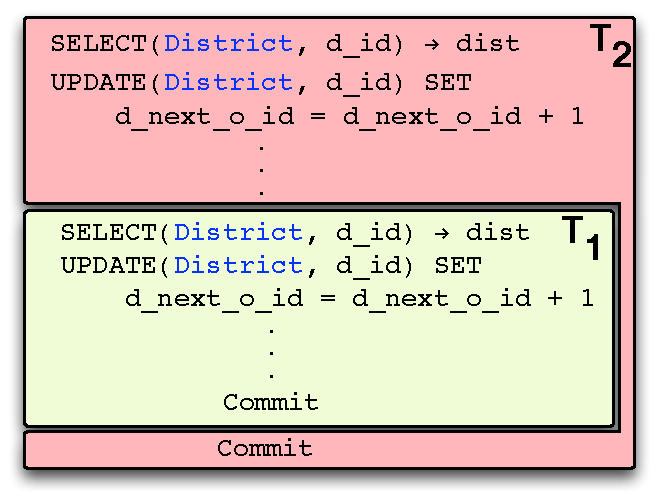
\includegraphics[scale=0.5]{Figures/motiv-eg-1-a}
}
%\hspace*{0.5in}
\subcaptionbox {
  RC Execution 2
  \label{fig:motiv-eg-1-b}
}{
  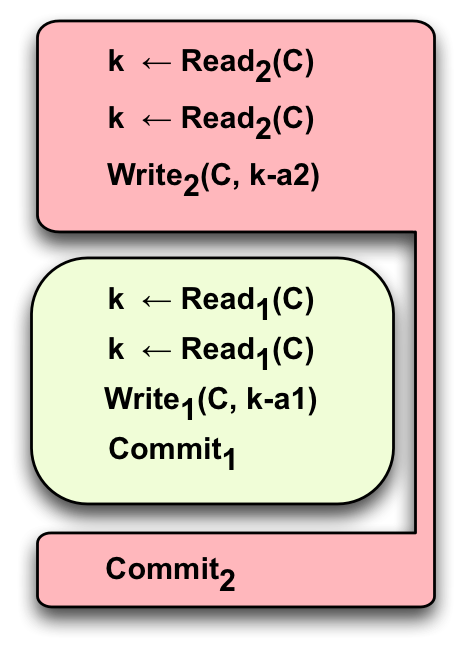
\includegraphics[scale=0.5]{Figures/motiv-eg-1-b}
}
\end{figure}
The figure depicts an execution as a series of read, write, and commit
operations.  The subscript of an operation indicates the transaction
that executes it\footnote{For clarity, the effects of different
transactions are shown in different colored backgrounds.} In the first
execution, transaction {\bf Wd1} reads the current balance (\C{k}) and
writes the new balance (\C{k-a1}), but before it commits transaction
{\bf Wd2} executes and commits, writing the new balance (\C{k-a2}). RC
isolation prevent {\bf Wd2} from witnessing the uncommitted writes of
transaction {\bf Wd1}.  Subsequently committing {\bf Wd1} leads to the
loss of {\bf Wd2}'s updates (the so called \emph{lost update
anomaly}~\cite{berenson}), resulting in an incorrect balance of
\C{k-a1}. The second execution describes a similar scenario with {\bf
Wd1} and {\bf Wd2} exchanging their roles.  Clearly, RC is not
sufficient because it loses the updates of one transaction resulting
in the violation of post condition.  We need an isolation level that
prevents lost updates.  \iso{Snapshot Isolation} (SI)~\cite{berenson}
fits this requirement by its definition. SI implementations
effectively serialize transactions that update a shared data object
mostly by aborting and re-executing a transaction if write-write
conflicts are detected during its commit.  Since SI, unlike SER, need
not necessarily rely on expensive lock-based concurrency control, it
is also more efficient, making it appropriate appropriate for both
`Wd' transactions. 

Thinking in terms of anomalies, as described above, is how database
programmers are often encouraged to reason about weak isolation.
Unfortunately, such reasoning does not rest on any sound foundation,
thus highly error-prone. Reasoning in terms of the implementations of
weak isolation is not any better since it requires application
programmers to understand and reason about low-level implementation
details of the database (or, databases) that are far removed from the
application semantics. An attractive alternative in this context is a
formal proof system that combines declarative reasoning about
isolation guarantees with operational reasoning about programs. We
demonstrate how our proof system makes this possible in the context of
the current example.

\begin{figure}
\centering
  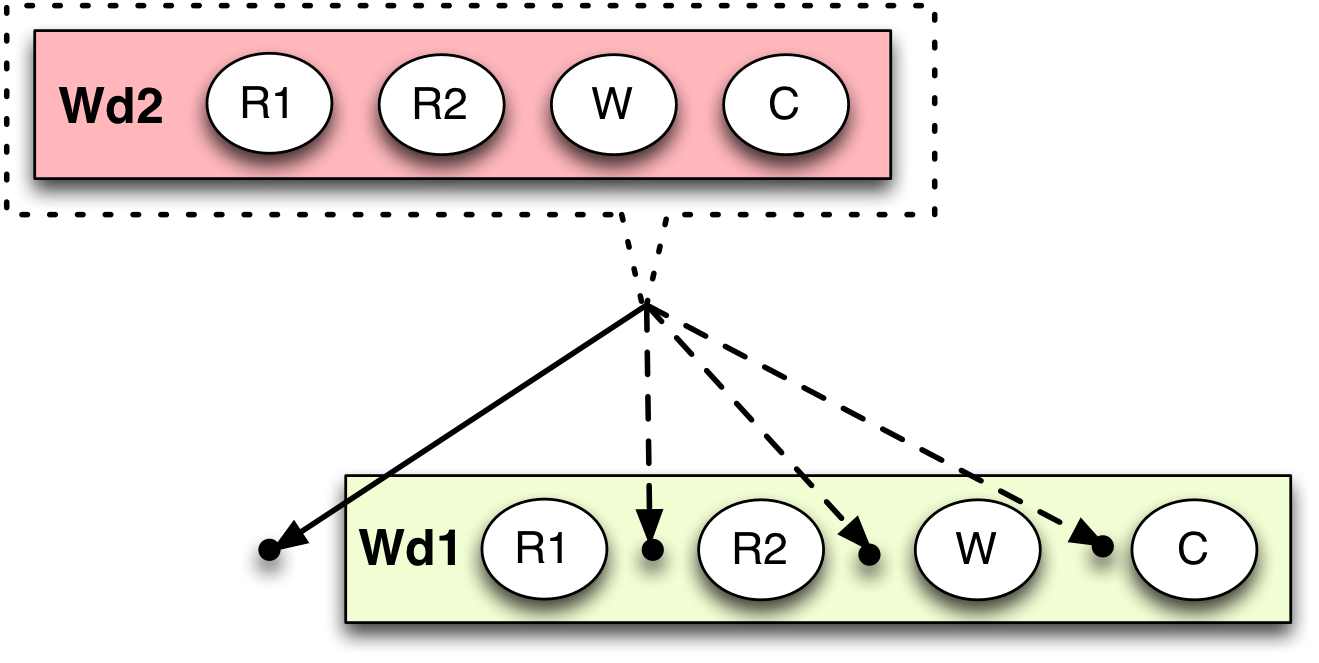
\includegraphics[scale=0.4]{Figures/motiv-eg-1-hb}

\label{fig:motiv-eg-1-hb}
\caption{$\hbZ$ arrows allowed by SI (solid) and RC (solid and dashed)
isolation levels for the example in Fig.~\ref{fig:motiv-eg-1}. Each
arrow represents $\hbZ$ relationship between all operations of `Wd2'
and operations in `Wd1' that follow the arrow head. Letters R, W and C
stand for read, write and commit, respectively.}
\end{figure}

Firstly, we note that the example in Fig.~\ref{fig:motiv-eg-1} is a
concurrent program, hence admits \emph{rely-guarantee} style
reasoning~\cite{rgjones}. Rely-guarantee is compositional proof
technique that allows us to reason about one thread at a time by
abstracting away the interference due to remaining threads
(collectively called \emph{the environment}) into a \emph{rely}
relation. In an ordinary concurrent program, every environment step is
a valid interference in the current thread. However, in presence of
transactions and variable isolation, determining what constitutes an
interference and what does not is a non-trivial problem. For example,
inside a serializable transaction no interference is a valid
interference, whereas inside a transaction executing under \iso{Read
Uncommitted}, the weakest isolation level, all interferences are
valid. Between these two extremes are various levels of isolation
that admit some interferences while prohibiting others. 
% For example, \iso{Read Committed} isolation admits interference of a
% committed transaction, but not that of an uncommitted transaction.
% \iso{Snapshot Isolation} admits interference from committed
% non-conflicting transactions, and so on. 
For the rely guarantee approach to be useful it has to constrain the
interference in accordance with the chosen level of isolation. The
first key observation we make is that we can constrain interference by
constraining the nature of \emph{happens-before} ($\hbZ$) relation
between transactions or their respective constituents. We make use of
the $\hbZ$ relation to axiomatize the interference characteristic of
isolation levels as their specifications ($\psi$). For example,
\iso{Read Committed} specification allows an operation $\eta_1$ of
$T_1$ to happen before an operation $\eta_2$ of $T_2$ only if every
operation in $T_1$ (including its commit) happens before $\eta_2$ (we
write $T_1 \hboar \eta_2$ to denote this). RC spec does not require
$T_1$ to happen before all operations of $T_2$, thus allowing it to
interfere in $T_2$, as possible under RC isolation. \iso{Snapshot
Isolation} spec requires two transactions that write to the same
variable to be related by happens-before.  This effectively proscribes
interference due to $T_1$ in $T_2$ (or, $T_2$ in $T_1$).
Formally\footnote{Note that specs are simplified for illustration. The
actual specs (\S~\ref{sec:opsem}) are more nuanced.  }:
\begin{smathpar}
\begin{array}{lcl}
\psi_{RC} & \defeq & \forall \eta_1,\eta_2,T_1,T_2.\; \txn(\eta_1) = T_1 
  \conj \txn(\eta_2) = T_2 \\
  & & \hspace*{0.6in}\conj T_1 \neq T_2 \conj \eta_1 \hboar
  \eta_2 \Rightarrow T_1 \hboar \eta_2 \\
\psi_{SI} & \defeq & \forall T_1,T_2.\; T_1 \neq T_2 \conj
  (\exists \C{X}.~{T_1 \wrstoar \C{X}} \conj 
                      {T_2 \wrstoar \C{X}})\\
  &  & \hspace*{0.6in}\Rightarrow{T_1 \hboar T_2} \disj {T_2 \hboar T_1} \\
\end{array}
\end{smathpar}
Fig.~\ref{fig:motiv-eg-1-hb} is a visualization of $\hbZ$ arrows
from `Wd2' to `Wd1' allowed by $\psi_{RC}$and $\psi_{SI}$. All
arrows re legal under $\psi_{RC}$ because in no case does an operation
$\eta_1$ from `Wd1' happen before $\eta_2$ of `Wd2' without the commit
of `Wd1' also happening before $\eta_2$. $\psi_{SI}$ however disallows
all dashed arrows, becase dashed arrows establish $\hbZ$ between `Wd2'
and only a subset of operations in `Wd1'. Ligher (blue) arrows with
hollow heads denote $\hbZ$ relationships that do not effect the value
of \C{C} in a way that causes the program to violate its
postcondition.  Darker (black) arrows with solid heads denote $\hbZ$
relationships that lead to the violation of postcondition. The task of
the reasoning framework is to determine if all $\hbZ$ relationships
allowed by an isolation level lead to the satisfaction of the
postcondition.

% There is a $\hb$ edge (first dashed) that is allowed by RC but
% prohibited by SI, which nonetheless does not lead to invariant
% violation. 

Specification of an isolation level encodes its interference
characteristic as constraints over $\hbZ$ relation. However, for this
to be useful in reasoning about programs, rely guarantee framework
should be able to use the specification to determine if an
interference is valid or invalid, allowing the programmer to only
focus on the former. Our second key observation is that this is
possible if the reasoning framework adequately tracks $\hbZ$ at each
program point, while preserving $\hbZ$ constraints as invariants
between program points. An interference that leads to the violation of
$\hbZ$ constraints (i.e., an invalid interference) is thus
automatically prohibited. For instance, consider the program point
after the write to \C{C} in `Wd1'. The expected invariant ($\phi$) at
that program point is shown below ($\committed$ stands for
``committed''):
\begin{smathpar}
\begin{array}{l}
  \neg\committed(\C{Wd1}) \conj (\neg\committed(\C{Wd2}) \Rightarrow
  \C{C = k-a1}) 
                \\
      \C{Wd1} \wrstoar \C{C} \conj (\committed(\C{Wd2})
                \Rightarrow \C{C = k-a1-a2})\}
\end{array}
\end{smathpar}
$\phi$ asserts that `Wd1' is not yet committed, and that it wrote to
\C{C}, and the value of \C{C} is either \C{k-a1-a2} or \C{k-a1}
depending on whether or not `Wd2' is committed. If $\phi$ stays
invariant until `Wd1' commits, then the postcondition (\C{C =
k-a1-a2}) can be established easily. However, an interference from
`Wd2' at this stage (captured by the last dashed arrow in
Fig.~\ref{fig:motiv-eg-1-hb}) may violate the invariant by writing
$\C{k-a1}$ to \C{C} and committing `Wd2', thus leading to
$\committed(\C{Wd2}) \Rightarrow \C{C=k-a2}$. Fortunately,
\iso{Snapshot Isolation} prevents this interference, and this can be
proved by showing that an interference from `Wd2' starting from a
execution state that satisfies $\psi_{SI} \wedge \phi$ leads to an
execution state where neither $\C{Wd2} \hboar \C{Wd1}$ nor $\C{Wd1}
\hboar \C{Wd2}$ holds (former does not hold because at least one write
from `Wd1' has happened before at least one operation of `Wd2', and
the latter doesn't hold because `Wd1' hasn't yet committed and `Wd2'
has already begun). Since `Wd2' also writes to \C{C}, this violates
the $\psi_{SI}$ constraint which we assume to be an invariant. A proof
for postcondition now follows from the contradiction. It is
informative to note that if the invariant is $\psi_{RC}$ instead of
$\psi_{SI}$, we cannot derive a contradiction and we cannot rule out
the interference, which causes (rightfully) the proof to fail.

We have thus far assumed an SC store that, in the absence of
transactions with special isolation requirements, makes effects of an
operation to be immediately visible to subsequent operations. Thus,
the natural behavior of SC store to totally order all operations w.r.t
$\hbZ$ relation could be in conflict with the constraints imposed by
weak isolation. To meet the requirements of weaker isolation levels,
say RC, the store has to adapt itself to \emph{hide} the effects of
concurrent transactions until they are committed. Once committed
though, the effects need to be immediately and perennially visible to
subsequent operations. This semantics of an SC store can be built into
the reasoning framework leading to a proof system tailor-made for such
stores. However, for the reasoning framework to be useful across the
stores, it has to be parametric over store consistency semantics, and
should be able to reconcile conflicts betweenconsistency and isolation
constraints. Later sections demonstrate how our reasoning framework
makes this possible.
